\documentclass[11pt,titlepage]{article}
\usepackage{geometry}
\geometry{
	a4paper,
	left=20mm,
	right=20mm,
	top=15mm,
	bottom=15mm,
}
\usepackage{tikz}
\usetikzlibrary{arrows,backgrounds}
\usepgflibrary{shapes.multipart}
\usepackage{graphicx}
\usepackage{mathtools}
\usepackage{inputenc}
\usepackage{amssymb}
\usepackage{wrapfig}
\usepackage[font=scriptsize]{caption} 
\linespread{1.0}
\usepackage{caption}
\renewcommand{\figurename}{Fig.}
\usepackage{subcaption}
\usepackage[title]{appendix}
\usepackage{enumitem}
\usepackage{listings}
\usepackage{xcolor}
\definecolor{codegreen}{rgb}{0,0.6,0}
\definecolor{codegray}{rgb}{0.5,0.5,0.5}
\definecolor{codepurple}{rgb}{0.58,0,0.82}
\definecolor{backcolour}{rgb}{0.95,0.95,0.92}

\lstdefinestyle{mystyle}{
	backgroundcolor=\color{backcolour},   
	commentstyle=\color{codegreen},
	keywordstyle=\color{magenta},
	numberstyle=\tiny\color{codegray},
	stringstyle=\color{codepurple},
	basicstyle=\ttfamily\tiny,
	breakatwhitespace=false,         
	breaklines=true,                 
	captionpos=b,                    
	keepspaces=true,                 
	numbers=left,                    
	numbersep=5pt,                  
	showspaces=false,                
	showstringspaces=false,
	showtabs=false,                  
	tabsize=2
}

\lstset{style=mystyle}
\setlength{\columnsep}{5pt}

%opening
\title{EECE6036: Intelligent Systems\\Homework \# 3}
\author{Zuguang Liu (M10291593)}



\begin{document}

\maketitle

\section{Neural Network Classifier with Hidden Layer}
\subsection{Problem Statement}

A classifier shall be implemented by a two-layer neural network to identify hand-written digits from MNIST dataset. The given MNIST dataset includes 5,000 labeled images, each of which writes digits `0' to `9' in different fashions, and is thus labeled into 10 classes. The images are represented by 28 $\times$ 28 pixels of normalized greyscale color values. 

\subsection{System Description}
Since neural network is a supervised learning model that requires training, there shall be an exclusive split of the dataset for training and testing. Consequently, apart from randomly shuffled, the data is also partitioned into 4,000 data points for training, and 1,000 for testing. The partitioning shall be stratified over the 10 classes, i.e., having the same number of data points for each class, in both the training set and testing set. In addition, the labels of the data are one-hot encoded to expand the output feature space to 10 dimensions. 

The two-layer neural network consists of a hidden layer and an output layer. \textbf{The hidden layer incorporates 128 neurons} that transfer all 784 pixel values of an image into a 128-dimensional feature space. Then the output layer uses this feature space to classify the image with an array of 10 elements, each of which represents the probability that the image can belong to a class. Hence the input and output of the network matches the images and labels in dimensions respectively. \textbf{Both layers use the \textit{sigmoid} activation function} (\ref{eqn:sigmoid}) \textbf{and a weight initialization scheme known as ``Xavier initialization''} showed in (\ref{eqn:xavier}), where $\mathcal{U}[a,b]$ is the uniform distribution in the interval $(a,b)$, $n_{in}$ is the input dimension of a layer, and $n_{out}$ is the output dimension of a layer \cite{glorot_understanding_nodate}

\begin{equation}
	f(x) = \frac{1}{1+e^{-x}}, \  f'(x) = f(1-f)
	\label{eqn:sigmoid}
\end{equation}

\begin{equation}
	W \sim \mathcal{U} \bigg[  -\sqrt{\frac{6}{n_{in}+n_{out}}} , \  \sqrt{\frac{6}{n_{in}+n_{out}}} \ \bigg]
	\label{eqn:xavier}
\end{equation}

The training of the model is done by back propagation repeated for multiple epochs. The training data is exclusively partitioned into 3,000 points for back propagation, and 1,000 points for validation. Within one epoch, all 3,000 points are shuffled, then used to adjust weights and biases. \textbf{The model is tested on the validation set every 10 epochs, resulting in a series of on-line training errors}. The error is calculated by (1 - balanced accuracy), where the balanced accuracy is the hit rate when comparing the true class and the predicted class using ``winner-take-all'' strategy over the output array. To further improve the training efficiency, several mechanisms are used in the training algorithm, including:
\begin{enumerate}[label=\alph*.]
	\item The gradient decent has an additional term to implement momentum, demonstrated in (\ref{eqn:bp_moment}), \textbf{where $\boldsymbol{\eta = 0.05$, $\alpha = 0.8}$, and $\boldsymbol{J}$ is loss function implemented by $\boldsymbol{J_2}$ loss}. 

	\begin{equation}
		\Delta w_{ij}(t) = -\eta \frac{\partial J}{\partial w_{ij}} + \alpha \Delta w_{ij} (t-1)
		\label{eqn:bp_moment}
	\end{equation}
	
	\item \textbf{Operating thresholds of 0.25 and 0.75 are used} so that output $\in [0, 0.25)$ is considered 0 when the corresponding truth is 0, and output $\in (0.75, 1]$ is considered 1 when the corresponding truth is 1. 
	
	\item Though the total repetition is 500 epochs, \textbf{an early stopping policy is used so that training stops when the on-line training loss does not improve for 50 epochs compared to the minimum loss over the whole training session}. As the validation set used for on-line testing is separate from the data used in back propagation, this ensures the model does not overfit the data. 
\end{enumerate}

After training, the resulting model is tested on the test dataset for analysis.

\subsection{Results}

Fig. \ref{fig:classifier_cm} (a) and (b) are confusion matrix that demonstrates the performance of the classifier on the training and testing dataset, respectively. Fig. \ref{fig:classifier_train} is show the change of the on-line training error over epochs. 

\begin{figure}[htb]
	\centering
	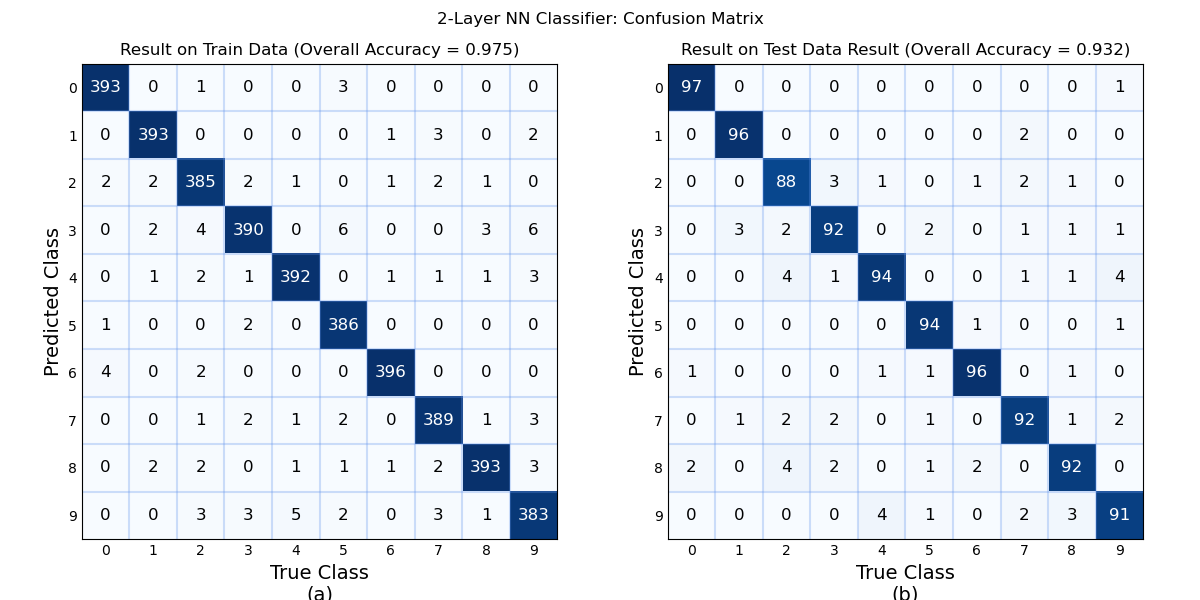
\includegraphics[width=\linewidth]{img/h3p1_cm}
	\caption{Confusion matrix of the classifier on the train data (a) and test data (b).}
	\label{fig:classifier_cm}
\end{figure}

\begin{figure}[htb]
	\centering
	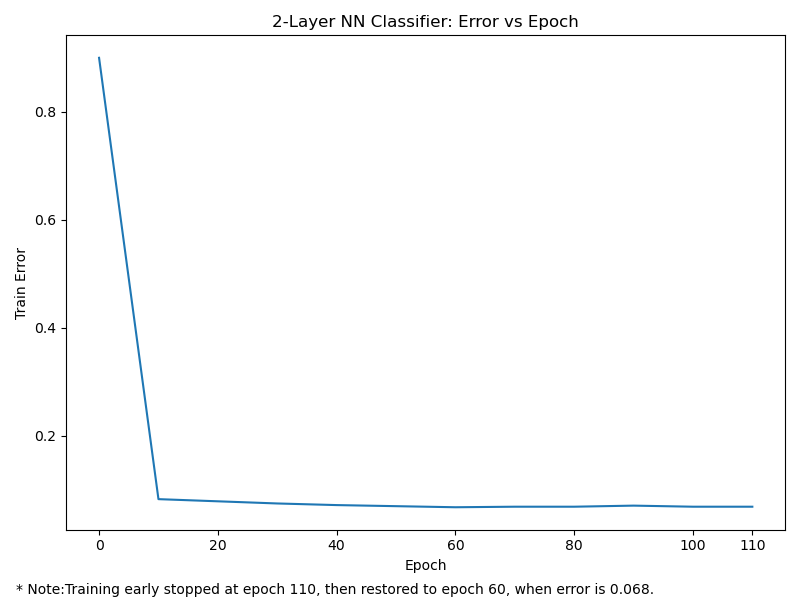
\includegraphics[width=0.6\linewidth]{img/h3p1_train}
\caption{The time series of the error (1-balanced accuracy) vs epochs.}
\label{fig:classifier_train}
\end{figure}

\newpage
\subsection{Analysis of Results}
The overall hit-rate on the train and test data is 98.2\% and 92.5\%, making the model a success. The 6.1\% difference could be caused by a slight level of overfitting, but both accuracy is good in general for a classifier. 

In the confusion matrices (Fig. \ref{fig:classifier_cm}), columns mark the actual class by the label, and rows mark the prediction from the model. In (b), since the test dataset are made so that there are 100 images for each `true class', the numbers in each column sums up to 100, so the numbers in the diagonal is the percent hit rate for each class. Images of classes `0', `1', `3', `5', `6', `7' have over 90\% hit rate for example, while other classes are also predicted well with the lowest hit rate at 88\%. Looking back into (a), we can find there are at minimum 391 correctly classified images for every class, which is still better than the worst result on the test data. Overfitting may have affected the result, but it could also be due to the way the digits are written has too many degrees of freedom and the classifier was not able to pick up all of them. 

To further improve the performance of the classifier, changes in several directions could be considered. 
\begin{enumerate}[label=\alph*.]
	\item Improvements on the quantity and quality of the data could be used. Quantitatively, the model could have larger number of data points for training and testing. Qualitatively, the images can be more defined in the resolution.
	\item The hyper-parameters of the model could be fully tested using grid search. 
	\item A more advanced optimization algorithm could be used during training. For example, instead of a single term to represent the first derivative of $\Delta w$ (\ref{eqn:bp_moment}), the \textit{ADAM} algorithm includes the second derivative also to further improve the efficiency of gradient descent.

\end{enumerate}

\newpage
\section{Neural Network Autoencoder with Hidden Layer}
\subsection{Problem Statement}

An auto-encoder network with one hidden layer shall be constructed for the same dataset, with the objective of reconstructing the image exactly. Therefore, the two-layer network has 784 inputs, and 784 outputs, representing a pixel in a 28 $\times$ 28 image. The number of perceptrons in the hidden layer should be the same as that of the one in the classifier. 

\subsection{System Description}

Since there are 128 neurons in the hidden layer of the classifier, the \textbf{autoencoder also has 128 hidden neurons}. The architecture of the autoencoder is similar to that of the classifier, except the output layer has 784 neurons to offer 784 values to regenerate the image. \textbf{Sigmoid (\ref{eqn:sigmoid}) and Xavier initialization policy (\ref{eqn:xavier}) are still used for both layers.} The training of the model also uses similar algorithm with minor modifications, including:
\begin{enumerate}[label=\alph*.]
	\item The input image and the ground truth used in the training are the same per step in the back propagation. 
	
	\item The back propagation uses \textbf{momentum-based gradient descent (\ref{eqn:bp_moment}) with $\boldsymbol{\eta = 0.01, \alpha = 0.8}$}.
	
	\item \textbf{The on-line training error is calculated by the average $\boldsymbol{J_2}$ loss function over all data points in the validation set.} This is presented by (\ref{eqn:j2}), where $N$ is the number of data points, $y_i^n$ and $\hat{y}_i^n$ are the original and predicted $i$-th pixel value on the $n$-th image, respectively. However, the same early-stop policy is used as well, so \textbf{the training will stop after no improvement on the error for 50 epochs}.
	\begin{equation}
		\bar{J_2} = \frac{1}{N} \sum_{n=1}^{N} J_2 = \frac{1}{1000} \sum_{n=1}^{1000} \bigg( \frac{1}{2} \sum_{i=1}^{784} (y_i^n - \hat{y}_i^n)^2 \bigg)
		\label{eqn:j2}
	\end{equation}
	
\end{enumerate} 

After training, the autoencoder is again tested on the test dataset for analysis.

\subsection{Results}
Fig. \ref{fig:autoenc_test} demonstrates the performance of the autoencoder overall and at each class, where the error is calculated by (\ref{eqn:j2}). The on-line training error vs epochs is shown in Fig. \ref{fig:autoenc_train}. 

\begin{figure}[htb]
	\centering
	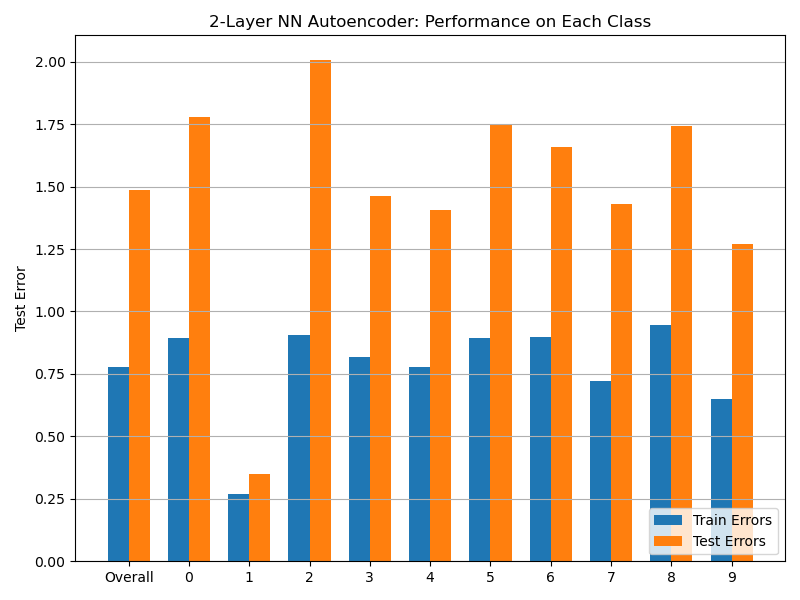
\includegraphics[width=0.6\linewidth]{img/h3p2_test}
	\caption{Performance of the autoencoder on the training and test set.}
	\label{fig:autoenc_test}
\end{figure}

\begin{figure}[htb]
	\centering
	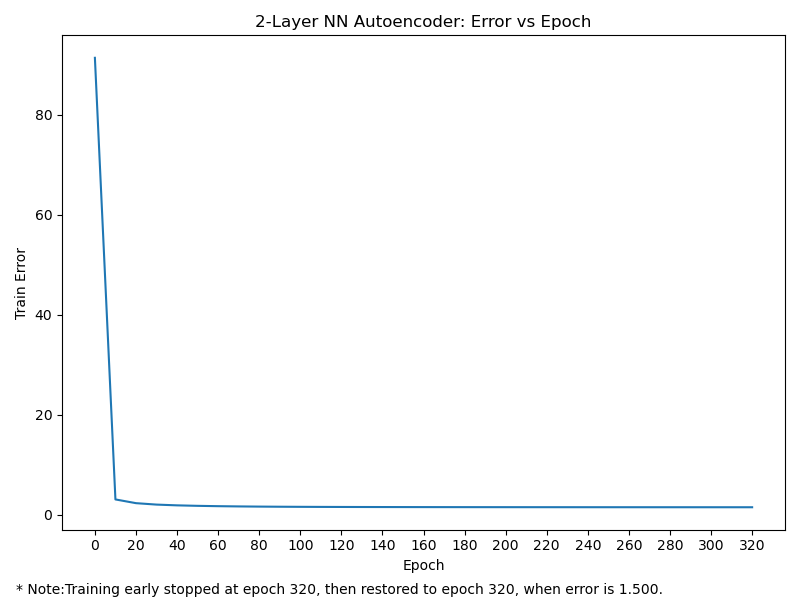
\includegraphics[width=0.6\linewidth]{img/h3p2_train}
	\caption{On-line training error vs training epochs over time}
	\label{fig:autoenc_train}
\end{figure}

\subsection{Features}

Weights of 20 neurons in the hidden layer of the classifier (Fig. \ref{fig:classifier_feature}) and the autoencoder (Fig. \ref{fig:autoenc_feature}) are normalized and illustrated by 28 $\times$ 28 images, as the feature space is 784-dimensional, in accordance to 784 pixels of the original images. Though neurons are chosen randomly, the selection of neurons in both model uses the same indexes, so that neurons in the same position are compared between the classifier and the autoencoder.

The original expectation was that the hidden features in the autoencoder could demonstrate more distinct shapes or patterns than the classifier, but the result suggests otherwise. It was surprising to see larger clusters of approximate pixel values in the classier features than in the autoencoder features. This is discusses further in the analysis.

\begin{figure}[htb]
	\centering
	\begin{minipage}{0.45\textwidth}
		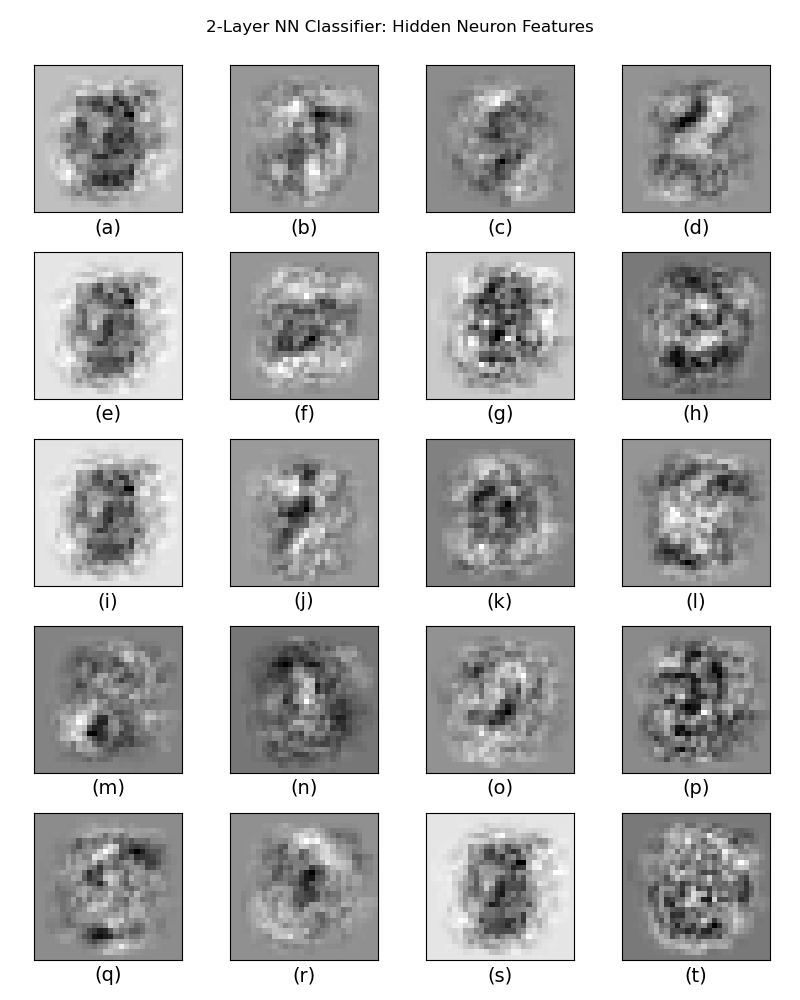
\includegraphics[width=\linewidth]{img/h3p1_feature}
		\caption{Feature map of 20 neurons in the hidden layer of the classifier network.}
		\label{fig:classifier_feature}
	\end{minipage}
	\hfill
	\begin{minipage}{0.45\linewidth}
		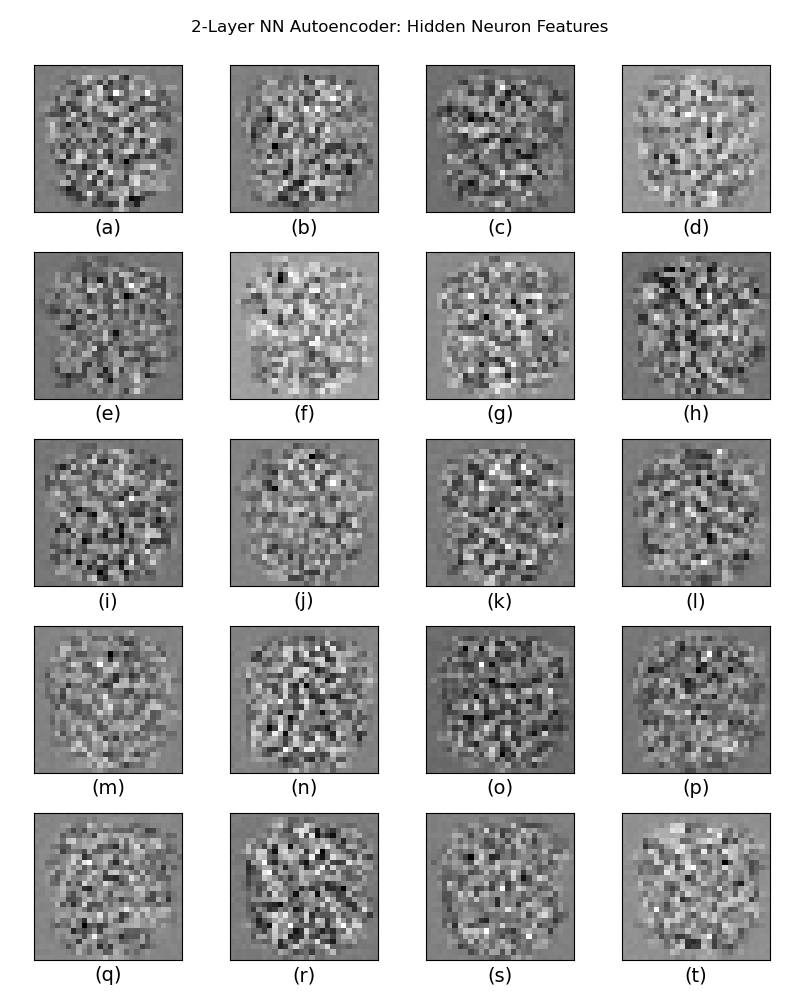
\includegraphics[width=\linewidth]{img/h3p2_feature}
		\caption{Feature map of 20 neurons in the hidden layer of the classifier network.}
		\label{fig:autoenc_feature}
	\end{minipage}

\end{figure}

\subsection{Sample Outputs}

Fig. \ref{fig:autoenc_output} demonstrates 8 reconstructed images (i)-(p) compared against the original images (a)-(h).

\begin{figure}[htb]
	\centering
	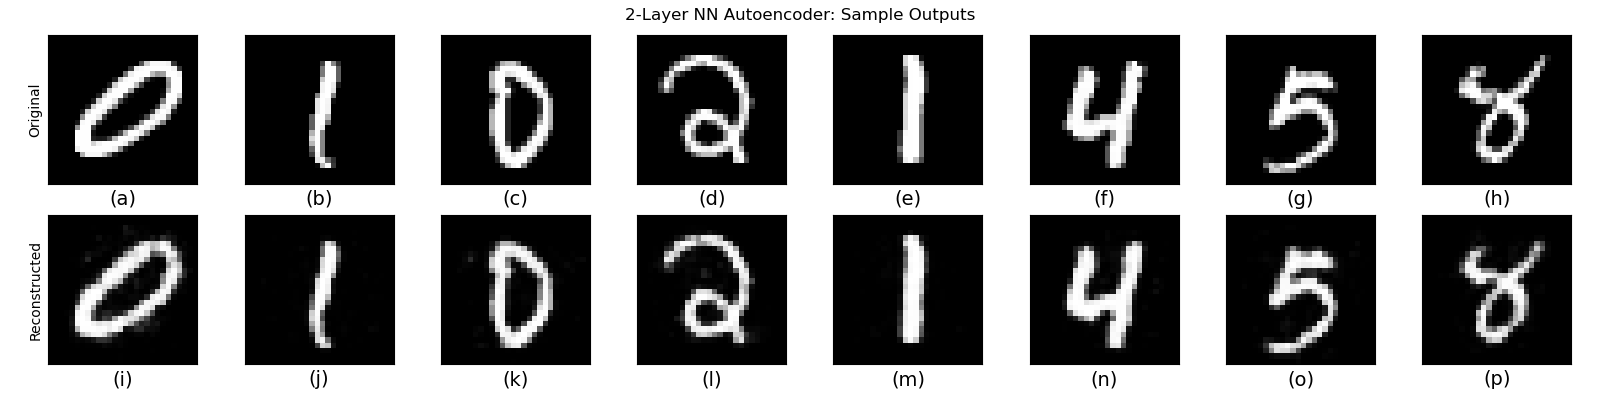
\includegraphics[width=\linewidth]{img/h3p2_outputs}
	\caption{8 Sample output of the autocencoder compared to original images.}
	\label{fig:autoenc_output}
\end{figure}

\subsection{Analysis of Results}

The resulting autoencoder is successfully trained with good level of accuracy. Mathematically, when the model is applied on the testing dataset, the overall $J_2$ error between the output and the original pixels is around 1.6 per image (Fig. \ref{fig:autoenc_test}), similar to the end on-line training error (Fig. \ref{fig:autoenc_train}). Visually, the reconstructed images look very much alike the original images (Fig. \ref{fig:autoenc_output}). From a detailed observation, there is minor noise in (p) that writes `2', (i) that writes `5' and (l) that writes `8'. This aligns with the $J_2$ loss in Fig. \ref{fig:autoenc_test}, as class 2, 5, and 8 have the highest errors among all classes. 

Though both classifier and autoencoder network do well in their own problems, the difference in the patterns of the hidden layer feature was quite astonishing at first. It is theorized that the checkerboard pattern in the autoencoder hidden features (Fig. \ref{fig:autoenc_feature}) is due to the need for the hidden layer to encode spatial correlations between pixels while reducing the feature space dimension. The model meets this goal by a set of weights that ``accepts'' some pixels ($w_{ij} > \boldsymbol{\bar{w}}$) and ``denys'' some pixels ($w_{ij} < \boldsymbol{\bar{w}}$) periodically at a certain ``sampling rate'', thus the checkerboard pattern. In the classifier (Fig. \ref{fig:classifier_feature}), however, there is no need to encode local correlations, so pixels that are spatially close are allowed to be weighted similarly, forming more visual clusters. Due to limited time and knowledge constraints, this hypothesis is not verified yet but may offer a reasonable explanation. 

Lastly, it is important that the training efficiently converges to such result, thanks to a well-defined model, detailed training policy (momentum-based gradient descent, early stop, etc.) and a finely-tuned set of hyper-parameters. The success of both models will provide an amount of experience in the future machine learning problems.

\vfill
\bibliography{refs}
\bibliographystyle{ieeetr}

\newpage
\begin{appendices}
\section{Python Code: preprocess.py}
\lstinputlisting[language=Python]{code/preprocess.py}

\newpage
\section{Python Code: nn.py}
\lstinputlisting[language=Python]{code/nn.py}

\newpage
\section{Python Code: p1\_train.py}
\lstinputlisting[language=Python]{code/p1_train.py}

\newpage
\section{Python Code: p1\_test.py}
\lstinputlisting[language=Python]{code/p1_test.py}

\newpage
\section{Python Code: p2\_train.py}
\lstinputlisting[language=Python]{code/p2_train.py}

\newpage
\section{Python Code: p2\_test.py}
\lstinputlisting[language=Python]{code/p2_test.py}

\end{appendices}

\end{document}